\section{Data}

The advent of mobile sensing techniques makes it possible to develop urban geography from social media source. Complement the conventional census, social media brings the benefit of larger sampling frequency and higher disaggregate in terms of space and time, which reaches a wide range of individuals as well as collects the movement in human inactive time, such as the mid-night.

In this work, we performed the demographical survey in Shenzhen, which is one of the most modern metropolis in China. The experiment is deployed on Wechat, a widely used social media application. Figure~\ref{fig:app} shows the data collecting interfaces. Each individual hands in his or her personal characteristics from social, economic and deomgraphic aspects. For privacy issue, all detailed personal information are desensitized to categorical levels (Figure~\ref{fig:app}(b)). Besides to those static features, each individual can upload dynamic traveling trips (Figure~\ref{fig:app}(c)). Each trip requires the information of start/end location and time, the traveling purpose and modes. To encourage the trip uploading, a credit system retains the contribution of individuals on trips and rewards those with the top credits (Figure~\ref{fig:app}(d)). 

\begin{figure}[htb!]
 \centering % avoid the use of \begin{center}...\end{center} and use \centering instead (more compact)
 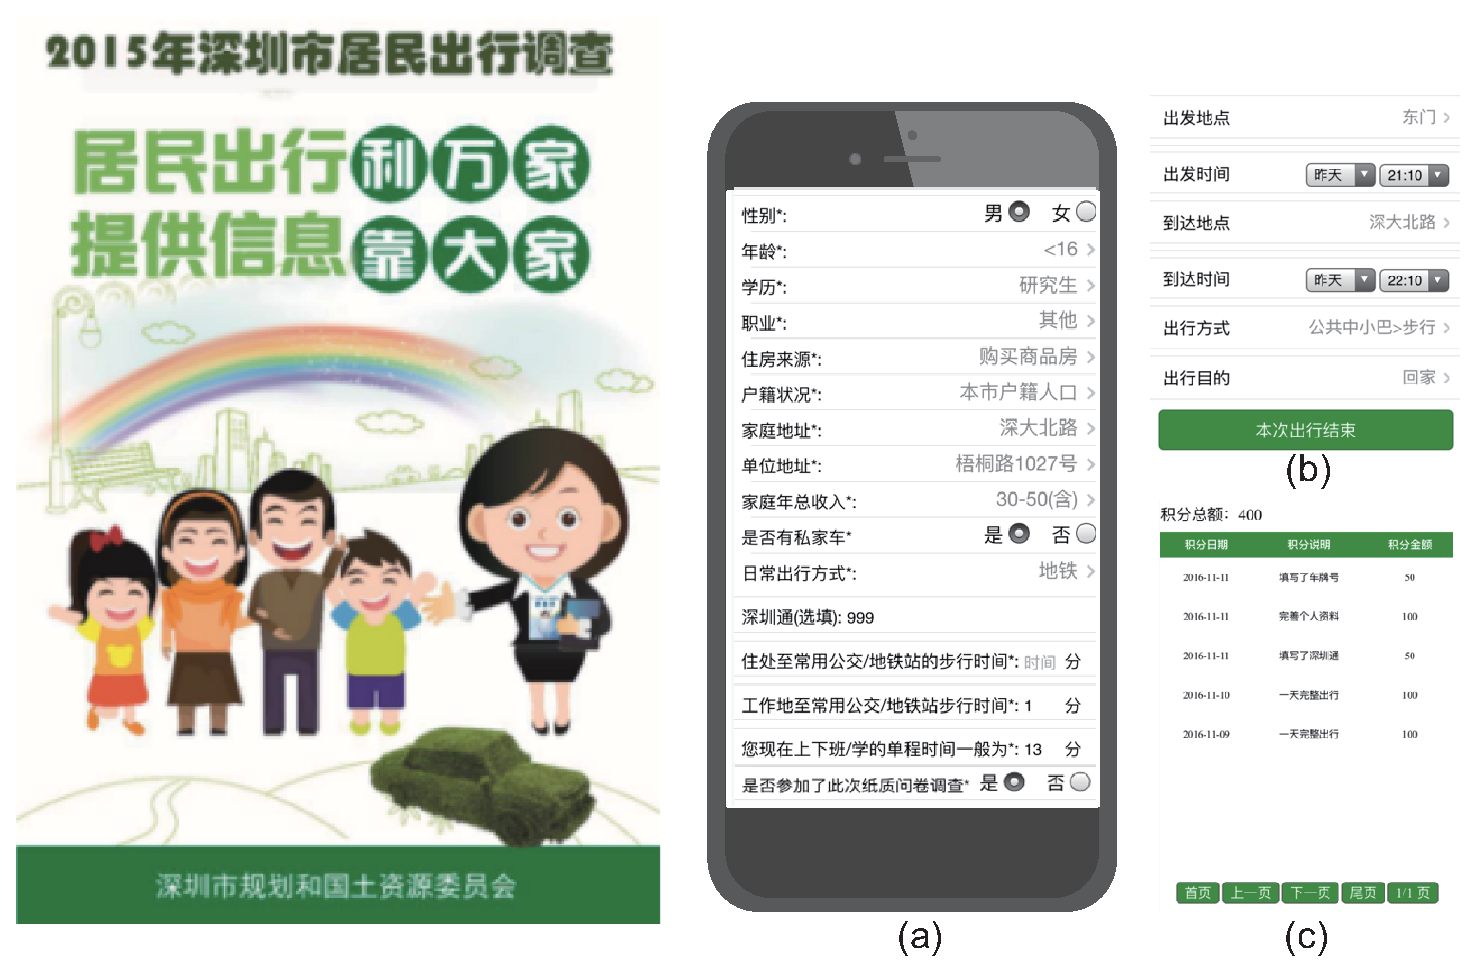
\includegraphics[width=\columnwidth]{pictures/survey_app}
 \caption{Collecting Interface: (a) welcome page; (b) personal characteristics collecting page; (c) trips collecting page; (d) credit system page}
 \label{fig:app}
\end{figure}

Over the releasing time period from June to October in 2015, 25481 individules (XX\% females and XX\% males)were reached and XXX trips are collected, XX trips per individual. Figure~\ref{fig:data_over} lists the XX variables, falling into 8 domains. Those domains give a generalized depiction of the individual characteristics and serve as the ingredients for the analysis of urban dynamics over diverse people. 

Considering the caveat that self-selecting individuals are most unlikely to represent any clearly defined population~\cite{Longley2015}, a series of preliminary statistics is performed to check whether it is rich enough to represent a wide range of human individuals in the city.


\begin{figure}[htb!]
 \centering % avoid the use of \begin{center}...\end{center} and use \centering instead (more compact)
 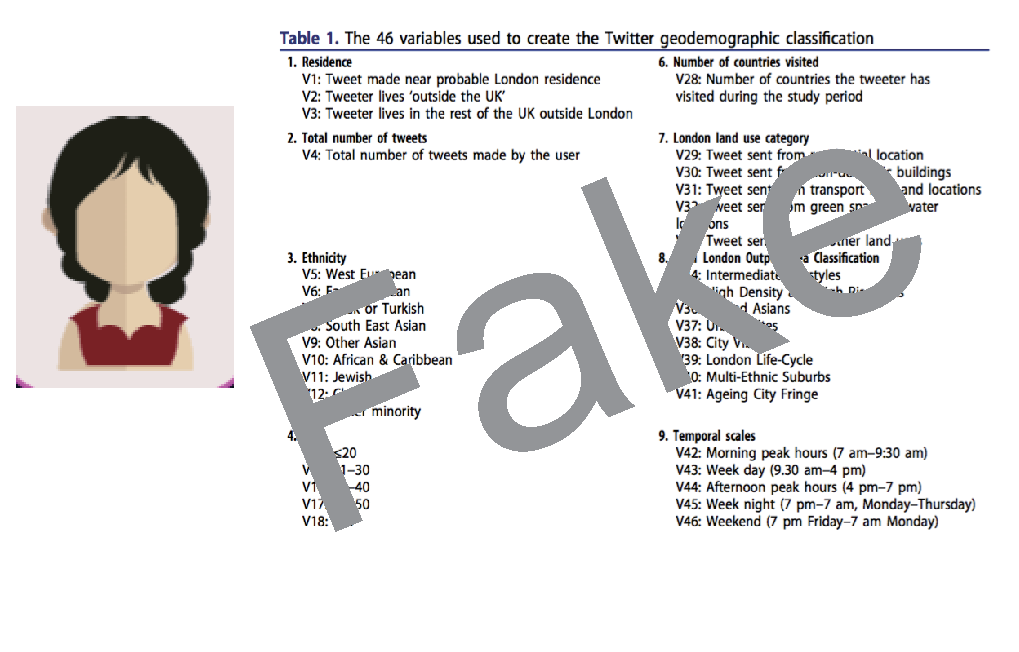
\includegraphics[width=\columnwidth]{pictures/data_over}
 \caption{Profile of Individual: XX variables falling into 8 domains enriches the analysis of urban dynamics}
 \label{fig:data_over}
\end{figure}

In the report (looking for some report), the penetration of mobile device is XXX, almost every XX people got a Mobile Phone in the urban. Figure~\ref{fig:data_age_edu} shows samples covering a wide range of all ages, dominately between 18 to 45. According to the 2015 Annual Census Statistics report~\footnote{http://www.sztj.gov.cn/xxgk/tjsj/pcgb/201606/t20160614\_3697000.htm}, people aging 15-64 occupy 83.23\% and the median age is 31.5. The distribution aligns to the fact that Shenzhen is a city where the majority is young people. The education levels is diverse from low to high. 



\begin{figure}[htb!]
 \centering % avoid the use of \begin{center}...\end{center} and use \centering instead (more compact)
 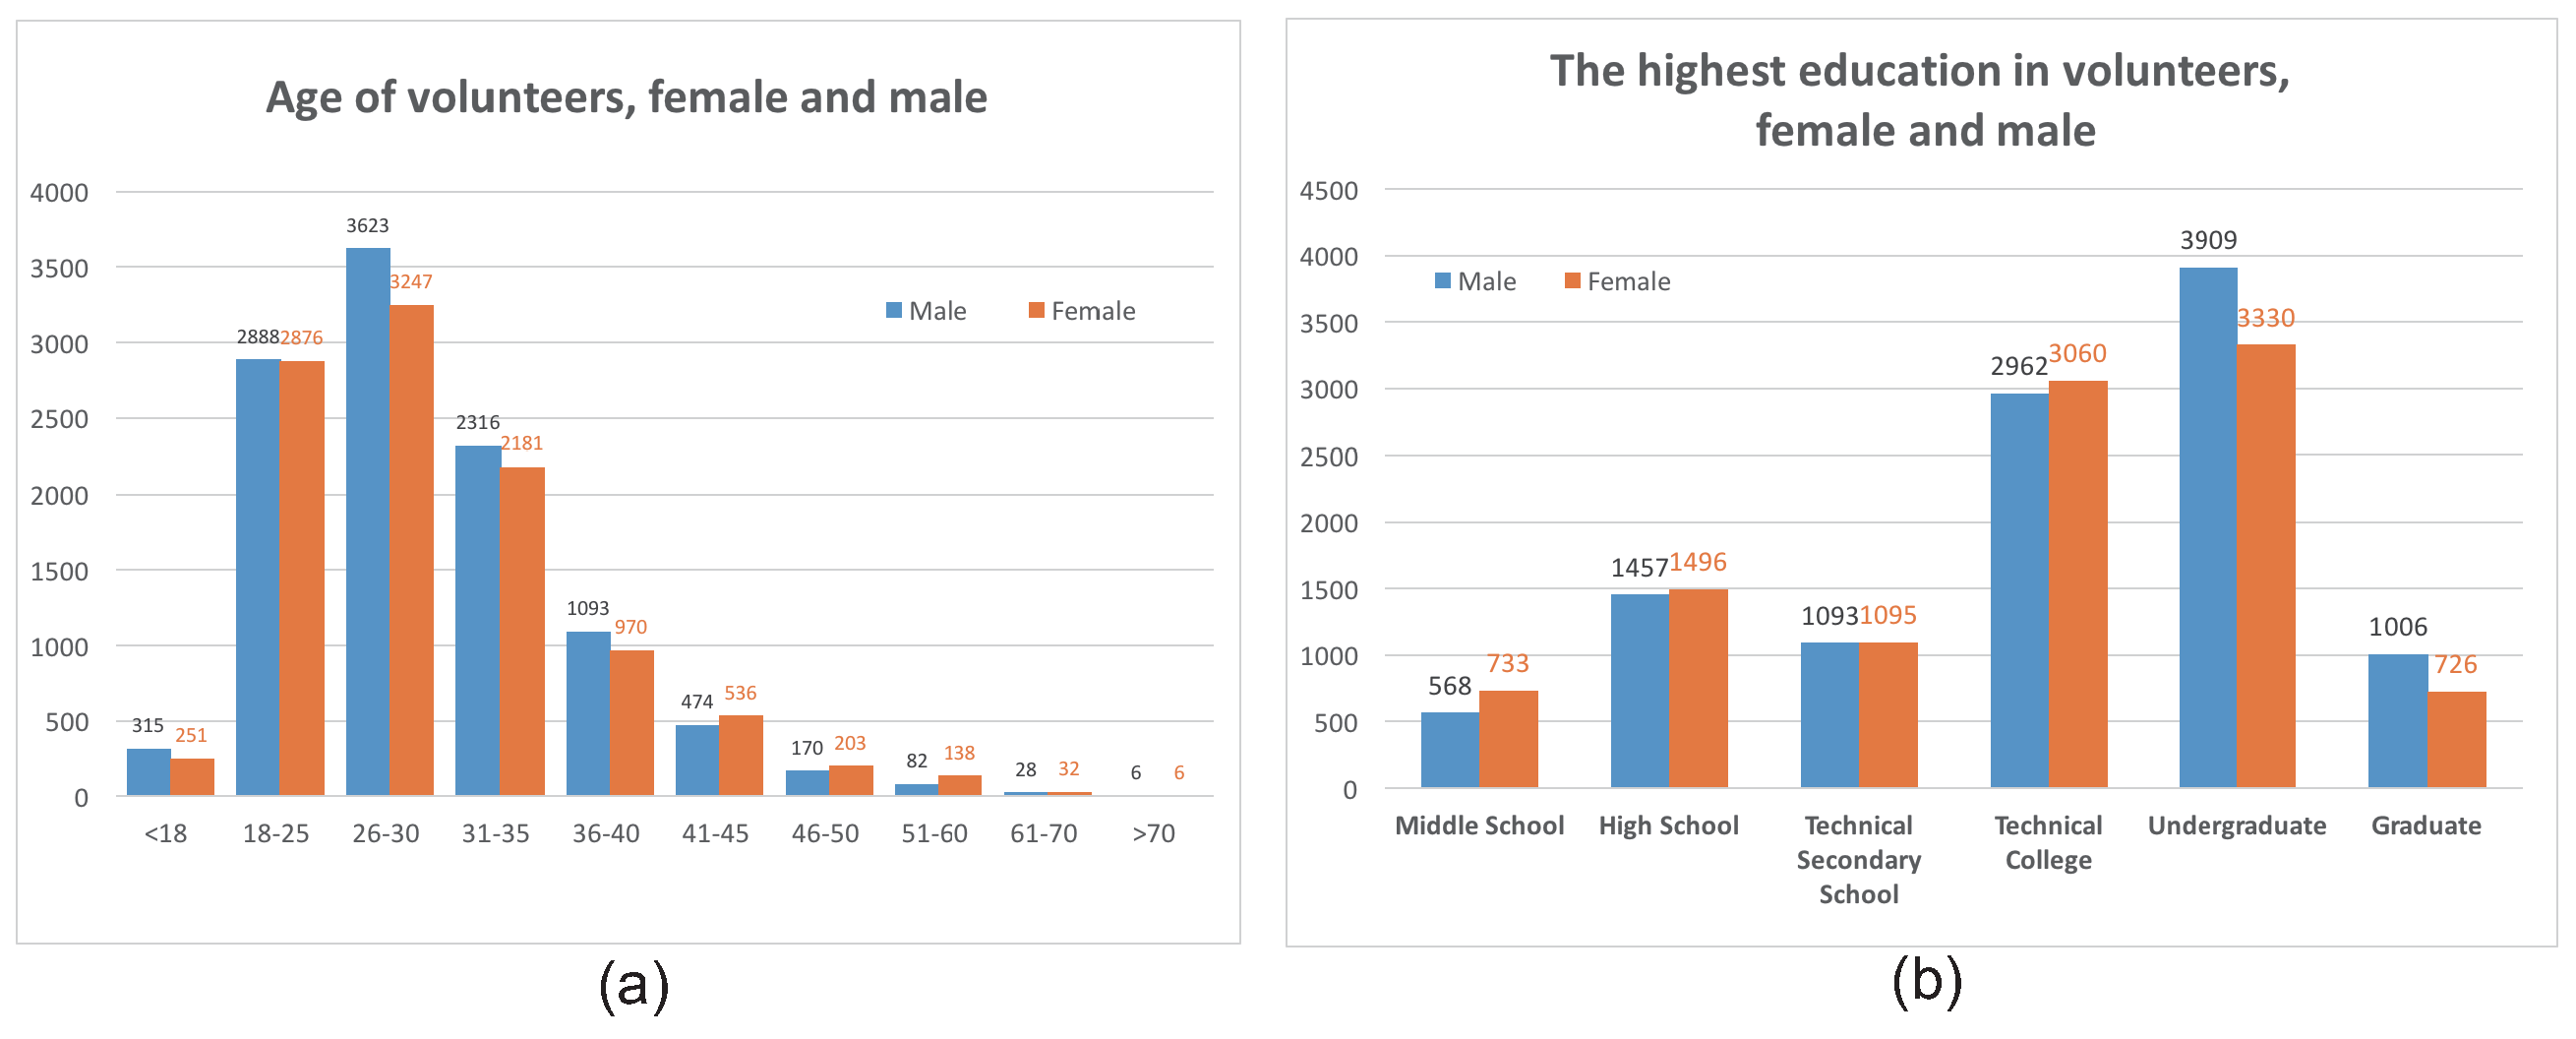
\includegraphics[width=\columnwidth]{pictures/data1}
 \caption{Evenly Distributed Age and Education: (a) age distribution; (b) education distribution}
 \label{fig:data_age_edu}
\end{figure}

As Figure~\ref{fig:data_job_inc} shows, the job types of sampling individuals includes the workers, officers, bussinessmen, which is very diverse. The yearly income various from the range from low to high.

\begin{figure}[htb!]
 \centering % avoid the use of \begin{center}...\end{center} and use \centering instead (more compact)
 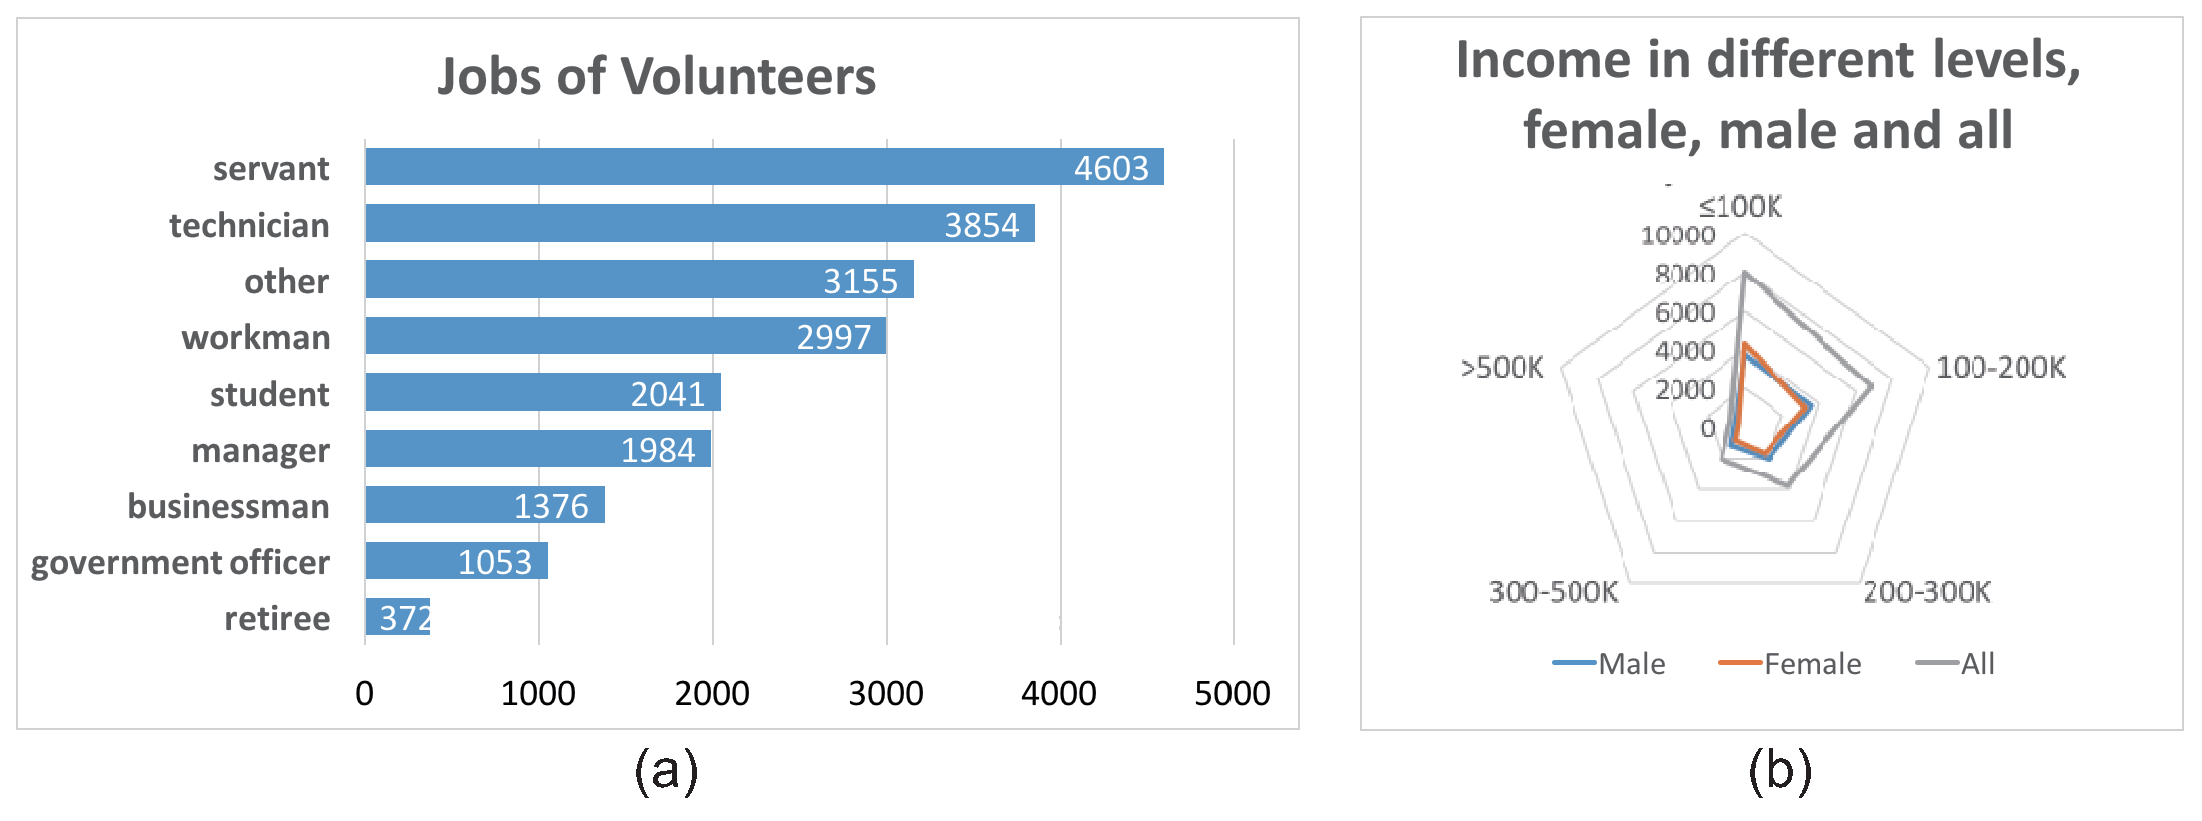
\includegraphics[width=\columnwidth]{pictures/data2}
 \caption{Diverse Job and Income Distribution: (a) job types; (b) income portion}
 \label{fig:data_job_inc}
\end{figure}


Figure~\ref{fig:data_geometry} shows the statistics of spatial activity. The activity time distribution in traveling obeys the commen sense. Morning and late afternoon peaks are detected in the data. The house distribution reports that our data has higher dense sampling in Futian, Nanshan districts, because those two are the most developed districts in Shenzhen.  



\begin{figure}[htb!]
 \centering % avoid the use of \begin{center}...\end{center} and use \centering instead (more compact)
 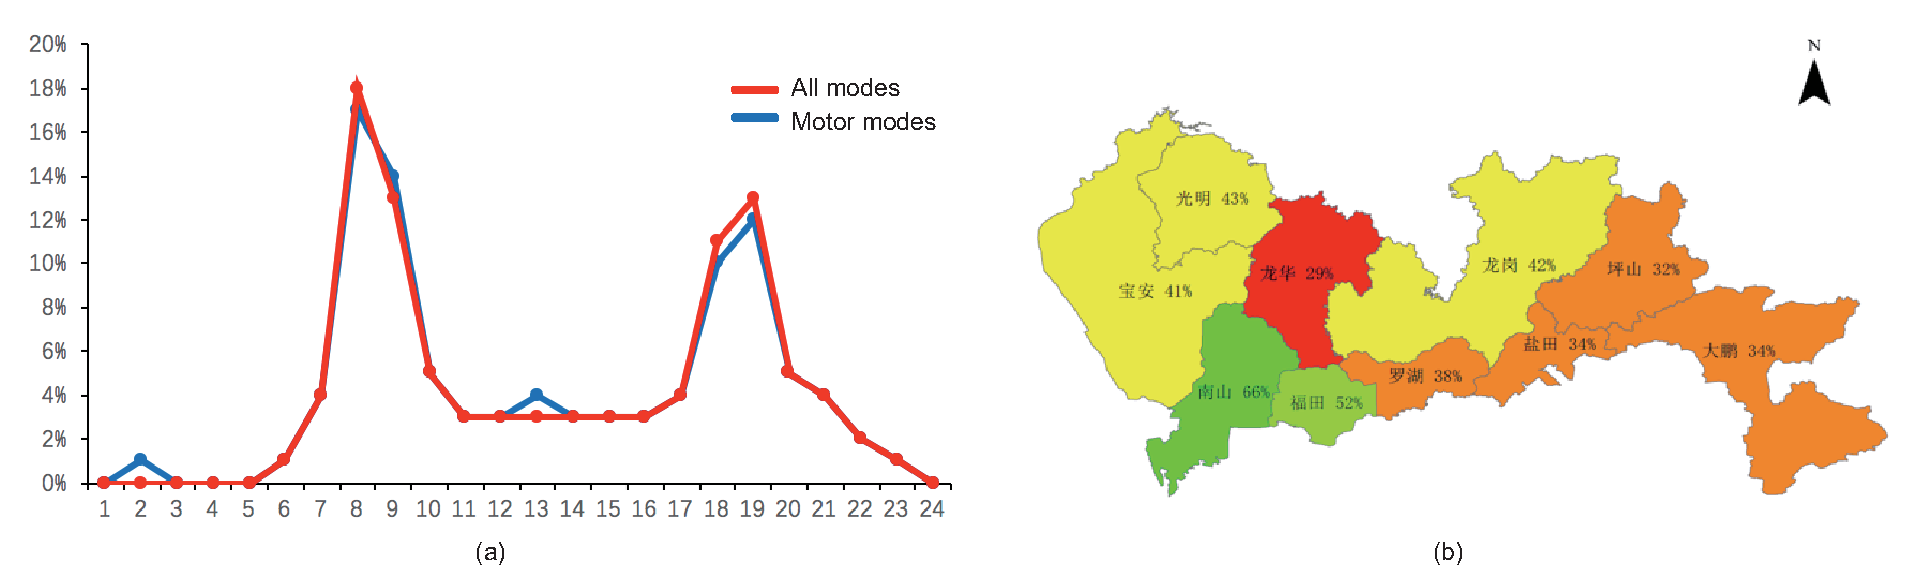
\includegraphics[width=\columnwidth]{pictures/data3}
 \caption{Statistical Overview of Social Characteristics}
 \label{fig:data_geometry}
\end{figure}


